\chapter{Existing Work and Literature}
This chapter starts off by presenting some of the existing algorithms and approaches to terrain rendering.
Afterwards, a selection of real-world systems are given, in which terrain LOD algorithms are used.

\section{Algorithms and Approaches for Terrain LOD}
Terrain LOD is a well-researched topic and over the last three decades, numerous approaches have been published.
In the following, some of the most important publications are listed in chronological order.
The approaches that are described in greater detail in the upcoming subsections are highlighted in \textbf{bold}:
\begin{itemize}
  \item ``Real-Time, Continuous Level of Detail Rendering of Height Fields'' \cite{lindstrom1996} by Lindstrom \textit{et al.} in 1996.
  \item \textbf{``ROAMing Terrain: Real-time Optimally Adapting Meshes''} \cite{roam} by Duchaineau \textit{et al.} in 1997.
  \item ``Real-Time Generation of Continuous Levels of Detail for Height Fields'' \cite{rottgerpaper} by Röttger \textit{et al.} in 1998.
  \item \textbf{``Fast Terrain Rendering Using Geometrical MipMapping''}  \cite{geomipmapping} by de Boer in 2000.
  \item ``Rendering Massive Terrains using Chunked Level of Detail Control'' \cite{chunkedlod} by Ulrich in 2002.
  \item ``Geometry Clipmaps: Terrain Rendering Using Nested Regular Grids'' \cite{geomclipmaps} by Hoppe and Losasso in 2004 and the follow-up \textbf{``Terrain Rendering Using GPU-Based Geometry Clipmaps''} by Asirvatham and Hoppe \cite{gpugeomclipmaps} in 2005.
  \item ``Continuous Distance-Dependent Level of Detail for Rendering Heightmaps (CDLOD)'' \cite{cdlod} by Strugar in 2009.
  \item \textbf{``Concurrent Binary Trees (with application to longest edge bisection)''} \cite{cbt} by Dupuy in 2020.
\end{itemize}
In the following subsections on the algorithms, all presented ideas are taken from their respective original publications,
unless noted otherwise.

\subsection{ROAM}
\textit{ROAM} (short for \textbf{R}eal-time \textbf{O}ptimally \textbf{A}dapting \textbf{M}eshes) 
is a terrain LOD algorithm developed by Duchaineau \textit{et al.} \cite{roam} published in 1997.
ROAM represents the terrain mesh using bintrees and performs triangle splits and merges
for generating and removing detail. Figure \ref{fig:roam} shows an example of 
a triangulation generated by ROAM.

\begin{figure}[H]
  \centering
  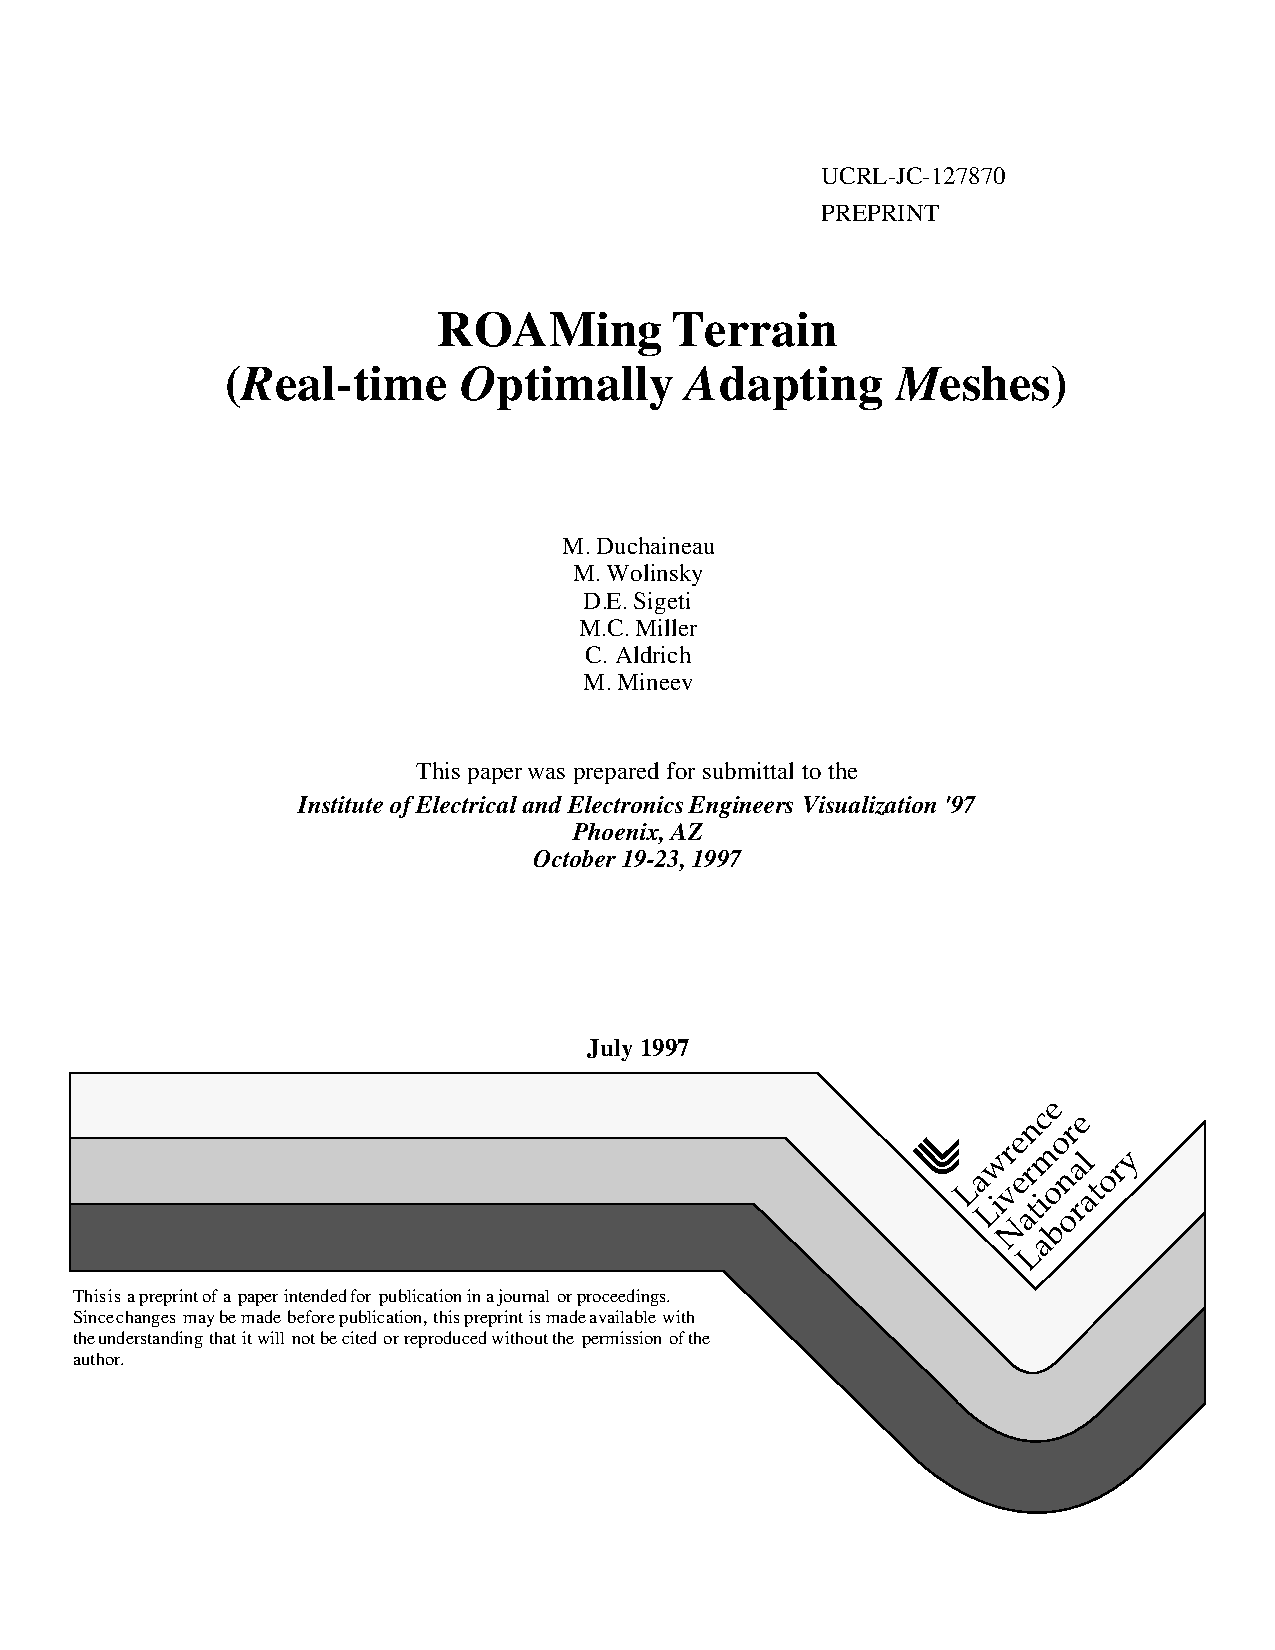
\includegraphics[width=0.7\textwidth]{roam}
  \caption{Top-down view of an example triangulation generated by ROAM (taken from \cite{roam}).}\label{fig:roam}
\end{figure}


The central idea of the algorithm is temporal coherence: between two frames, 
the meshes are often very similar. This means that the mesh from a previous frame can be used to compute 
the mesh of the current frame, rather than building up the mesh from ground up.
This is done using two priority queues: a split queue $\mathcal{Q}_s$ and a merge queue $\mathcal{Q}_m$.
The split queue contains splittable triangles $T$
and the merge queue contains mergable triangle pairs $(T,T_B)$.
At each frame, the terrain mesh gets split and merged using $\mathcal{Q}_s$ and $\mathcal{Q}_m$. until either the required size/accuracy is reached
or the time runs out. 
The splits and merges always result in a continuous mesh, i.e. the mesh cannot contain any 
T-junctions.
The elements of $\mathcal{Q}_s$ and $\mathcal{Q}_m$ are ordered by 
various geometric error metrics, some of which are the following:
\begin{itemize}
  \item Nested bounding volumes named \textit{wedgies}, which are defined to include the entire $x$ and $z$ extent of a triangle and its subtriangles 
        plus some padding space above and below the highest and lowest points respectively. Wedgies are computed while building the initial mesh at the beginning of the algorithm.
  \item Another metric is the geometric screen distortion, i.e. the distance between where a node is supposed to be on the screen and where the algorithm actually places the node.
        The maximum of all distances is calculated and used as the base priority metric of the algorithm.
\end{itemize}

While the bintree trees gets traversed, various flags are updated which indicate whether a wedgie is inside the view-frustum completely, partially or not at all
and based on these flags, bintree children outside of the view-frustum do not get recursively descended.


\subsection{GeoMipMapping}
\textit{Geometrical Mipmapping (GeoMipMapping)} is a terrain LOD approach published by de Boer \cite{geomipmapping} in the year 2000.
The central idea of GeoMipMapping is its analogy to texture mipmapping: just like how textures of far away objects are rendered using lower resolution texture mipmaps,
terrain areas that are far away from the camera should also be rendered with a lower resolution mesh.

This is achieved by splitting up the terrain into so-called \textit{blocks} (also called \textit{patches}) of a fixed side length $2^n + 1$ for some $n \in \mathbb{N}$.
Each block has a LOD level $0\leq l \leq n$ that changes dynamically at runtime.
Each representation of a block at a specific LOD level is called a \textit{GeoMipMap}.
For each GeoMipMap, the number of vertices on one side is $2^{l}+1$ and the number of quads is $2^{2l}$.
Figure~\ref{fig:geomipmapping-patch-example} shows an example of a $5 \times 5$ block at LOD levels 2, 1 and 0.

\begin{figure}[H]
  \centering
  \subfloat[\centering LOD level 2 (maximum).]{{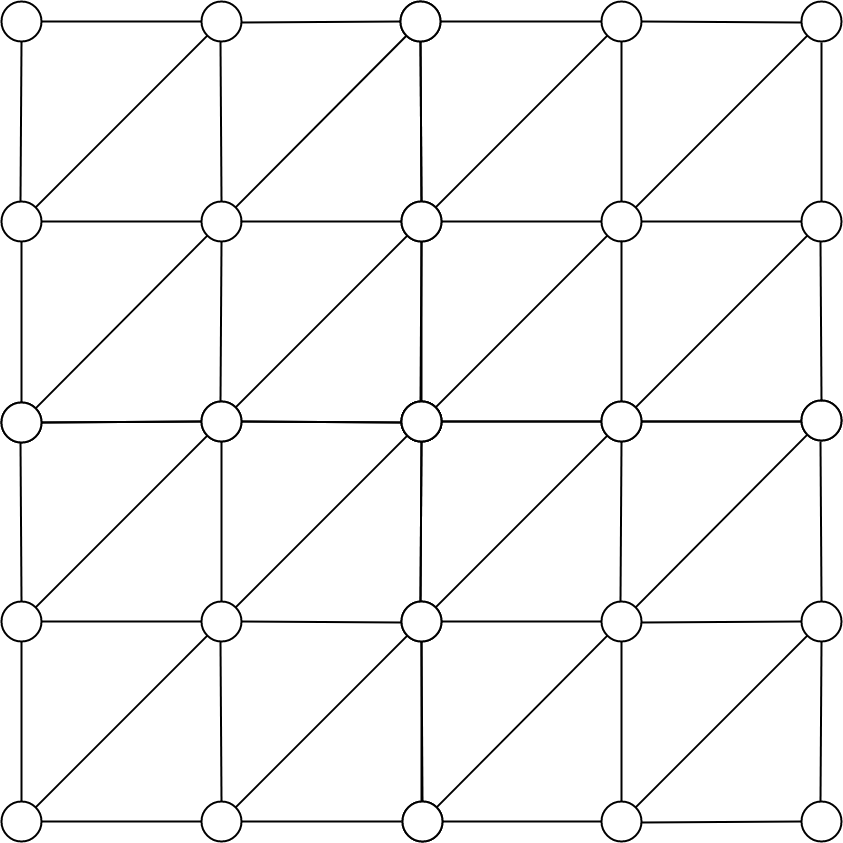
\includegraphics[width=0.28\textwidth]{geomipmapping-level-2.png} }}
  \qquad
  \subfloat[\centering LOD level 1.]{{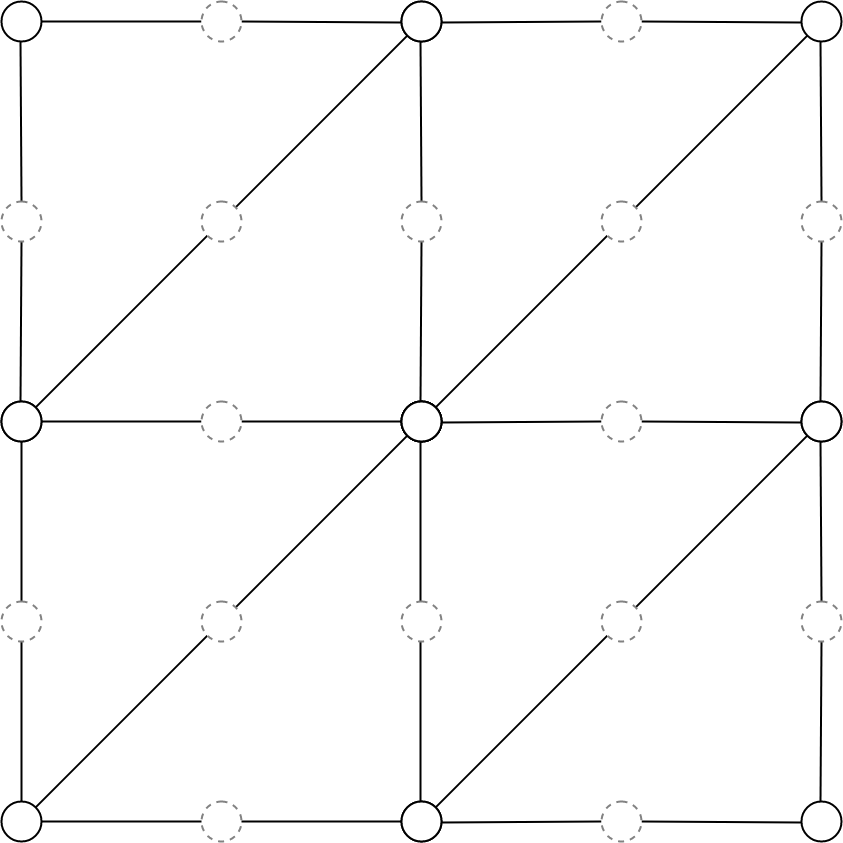
\includegraphics[width=0.28\textwidth]{geomipmapping-level-1.png} }}
  \qquad
  \subfloat[\centering LOD level 0 (minimum).]{{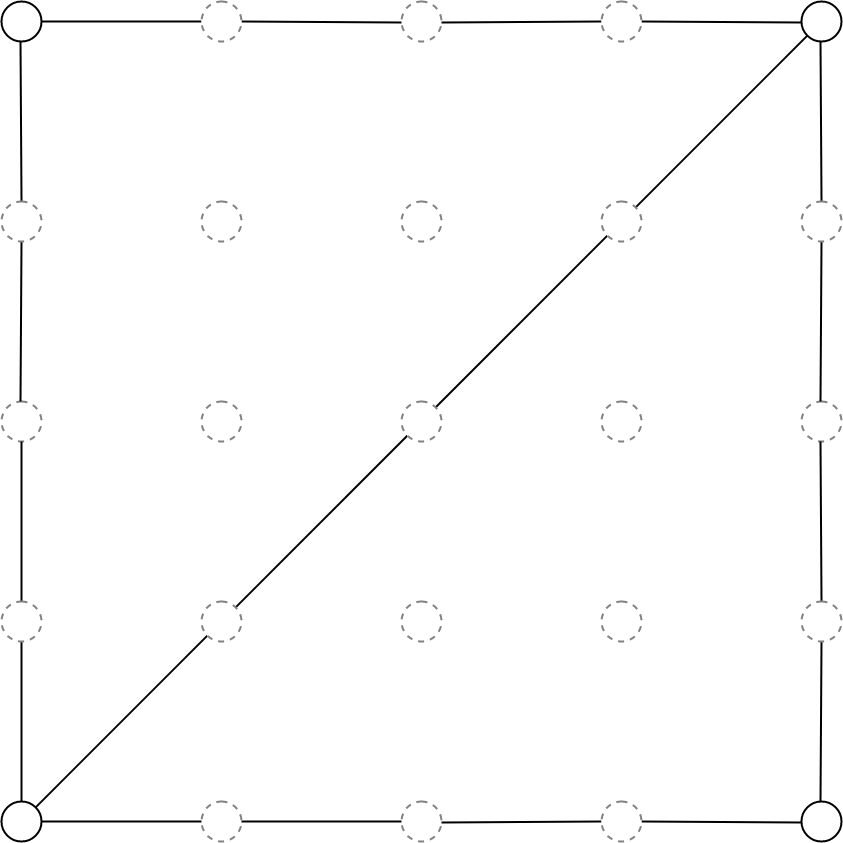
\includegraphics[width=0.28\textwidth]{geomipmapping-level-0.png} }}
  \caption{Example of each GeoMipMap of a $5 \times 5$ block. The omitted vertices of lower LOD GeoMipMaps are marked as dotted circles (based on \cite{geomipmapping}).}\label{fig:geomipmapping-patch-example}
\end{figure}

The organisation of the terrain into blocks allows for easy view-frustum culling, which is performed 
with a quadtree, where each node contains the AABB of its four children and the leaf nodes 
contain the actual blocks.

The LOD level for each block is selected at runtime and is based on the 
screen-space error that is caused by changing the LOD level of a block.
When the LOD level of a block changes, vertices get added or removed from the block,
which causes a difference in height $\delta$ between the two GeoMipMaps of that block. Projecting $\delta$ into 
screen-space yields $\varepsilon$. 
This $\varepsilon$ can be limited with a threshold $\tau$, such that 
the change in LOD level occurs only if $\varepsilon < \tau$.
The LOD selection can be sped up by pre-computing $\varepsilon$ per GeoMipMap and storing it in a look-up table.

GeoMipMapping avoids cracks by checking the four neighboring blocks
of a block and omitting the vertices that would cause cracks in the terrain.
The vertex omission is performed by rendering the bordering row/column of the current block
as triangle fans, as shown in figure~\ref{fig:geomipmapping-crack-avoidance}.

\begin{figure}[H]
  \centering
  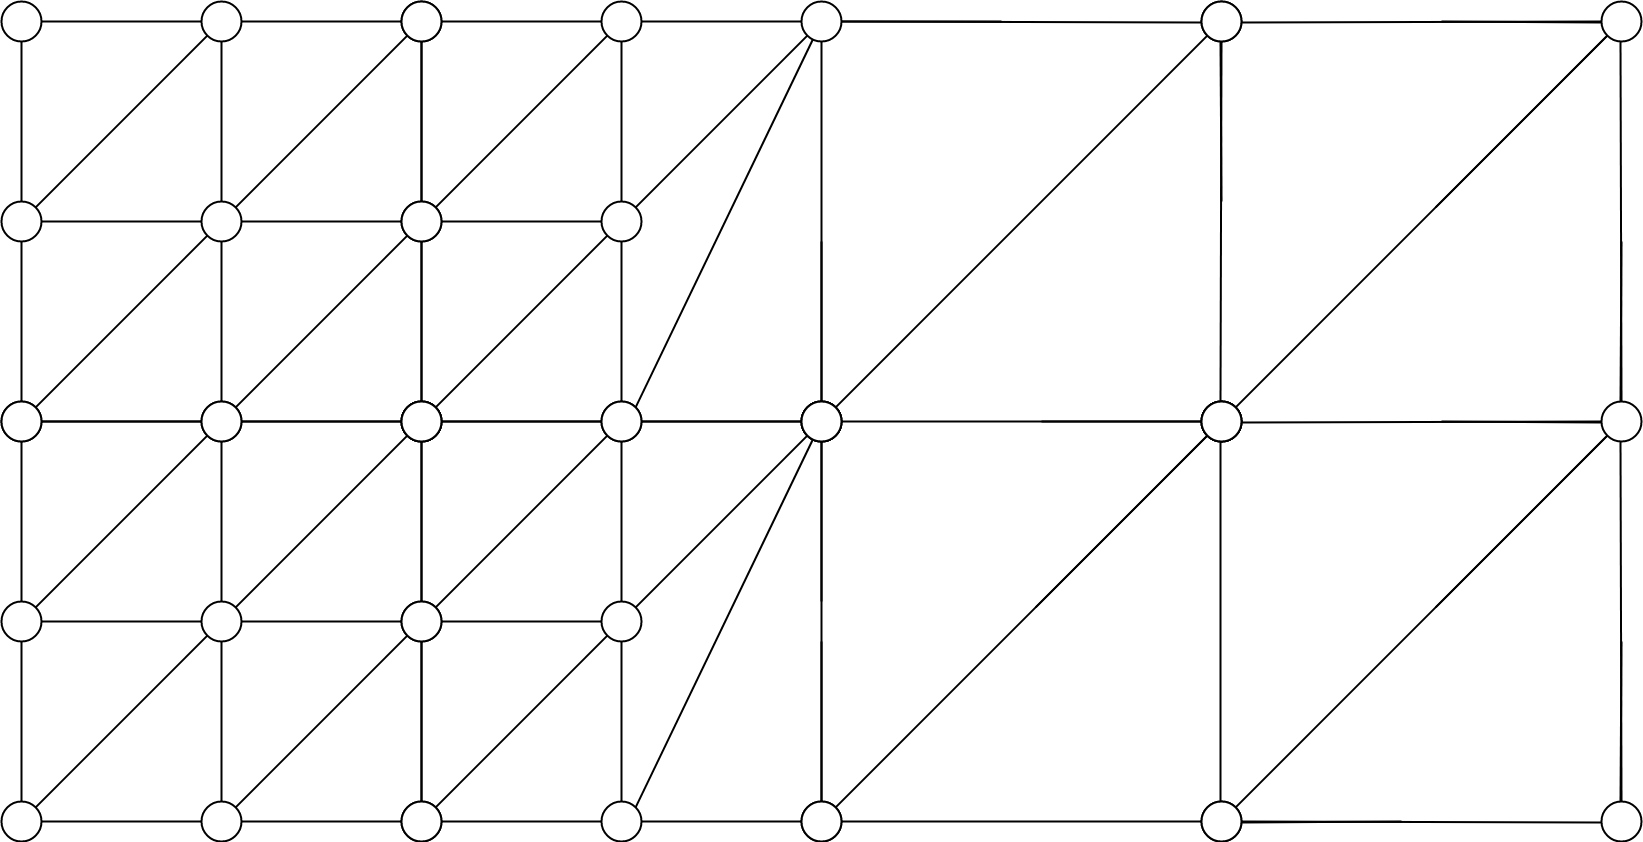
\includegraphics[width=0.7\textwidth]{geomipmapping-crack-avoidance}
  \caption{Example of GeoMipMapping's crack avoidance between a LOD 2 and a LOD 1 GeoMipMap of two $5 \times 5$ blocks (based on \cite{geomipmapping}).}\label{fig:geomipmapping-crack-avoidance}
\end{figure}

Some further optimizations that were mentioned, which extend the just described basic GeoMipMapping algorithm, 
are \textit{trilinear GeoMipMapping} (i.e. morphing the vertices at LOD transitions similarly to trilinear mipmapping),
and \textit{progressive GeoMipMap streaming}.

\subsection{(GPU-based) Geometry Clipmaps}
Geometry Clipmaps \cite{geomclipmaps} is a terrain rendering technique published by Hoppe and Losasso in 2004.
A follow-up GPU-based variant of Geometry Clipmaps \cite{gpugeomclipmaps} was published in GPU Gems 2 by Hoppe and Asirvatham in 2005.
In this section, the basic features of the GPU-based Geometry Clipmaps algorithm are described,
and we leave out some more advanced features, such as compression and noise-generated details.

The algorithm is based on a single flat mesh centered around the camera.
The flat mesh is organized as a set of nested rings of $l$ levels, 
where the innermost level $l-1$ is a filled-in $n \times n$ grid, and where the ring at level $i$ is twice as big as the ring 
at level $i + 1$. This $n$ must be of the form $2^k - 1$ for some $k \in \mathbb{N}$. 
Each ring at a level is organized into 12 blocks of size $m \times m$, where $m = (n+1)/4$.
Gaps inbetween the blocks are filled up with special types of blocks, namely the $m \times 3$ \textit{ring fix-up} and the $(2m+1) \times n$ \textit{interior trim}.
In order to avoid T-junctions, a string of degenerate triangles is rendered at the border between blocks of 
different size. Since each block is identical up to translation and uniform scale, they get stored once on a vertex and index buffer 
and translated and scaled in the vertex shader at runtime, which greatly reduces memory consumption.
Figure \ref{fig:geometry-clipmaps-mesh} shows an example of this mesh. 

\begin{figure}[H]
  \centering
  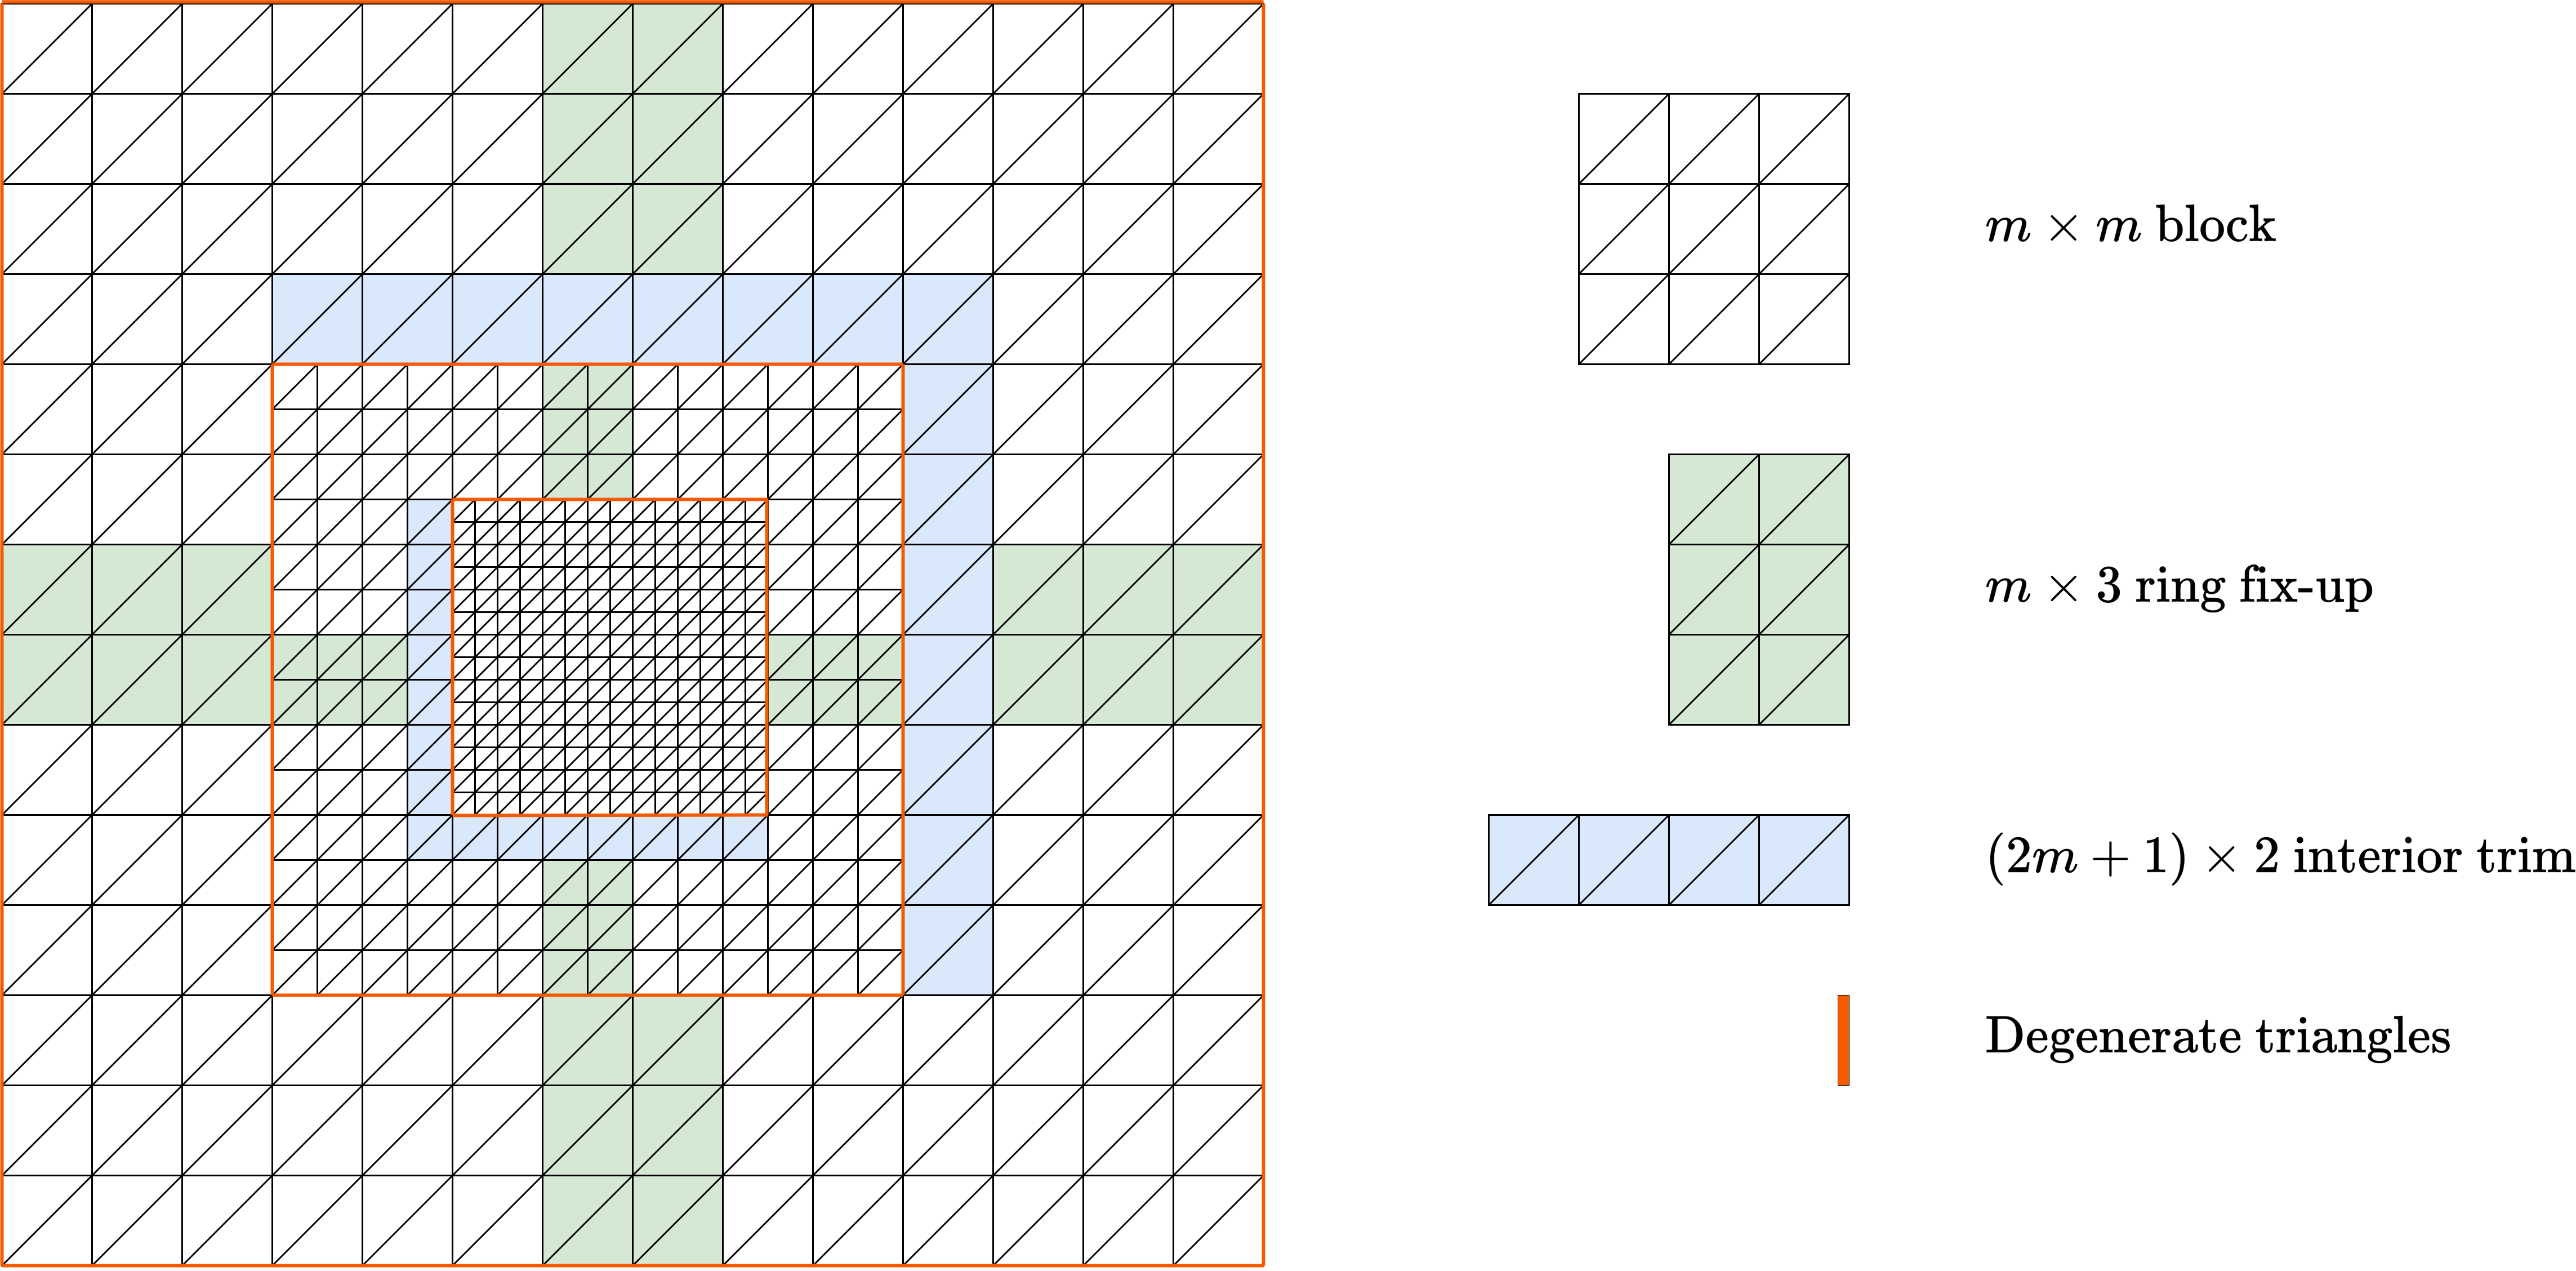
\includegraphics[width=1.0\textwidth]{geometry-clipmaps-mesh}
  \caption{Example of the flat mesh in Geometry Clipmaps with $n = 15$, $m = 4$ and $l = 3$ (based on \cite{gpugeomclipmaps}).}\label{fig:geometry-clipmaps-mesh}
\end{figure}

In the vertex shader, the algorithm samples the height values from the heightmap texture.
Additionally, it performs the calculations for the so-called \textit{transition regions}, 
which are regions near the border of two levels in which 
the levels get morphed, so that the transition between levels is smooth and no popping occurs.
The morphing is performed by computing the blend factor $\alpha$,
which is based on the position of the camera and the position of the vertex in world-space.
This factor $\alpha$ is defined such that it is 0 everywhere except at the transition region,
where it linearly grows from 0 to 1 until reaching the border.

During rendering, view-frustum culling is performed by intersecting each block with the view-frustum,
and if the AABB of the block does not intersect the view-frustum, it does not get rendered.

Shading is performed with a normal map, which has twice the resolution of the heightmap.

\subsection{Concurrent Binary Trees}
The \textit{concurrent binary tree (CBT)} \cite{cbt} is a data structure published by Dupuy in 2020.
It essentially allows for binary trees to be computed in parallel using a binary heap 
represented as a bitfield. This allows for easy concurrent manipulation of tree nodes using bitwise operations.
The data structure is applicable to problems relying on binary trees, 
such as the \textit{longest edge bisection}.

The paper contains a section which describes the application of CBTs to terrain rendering.
The approach is similar to \cite{roam} in the sense that it computes a triangulation of the terrain using bintree splitting and merging.
The main difference is that the spliting and merging of the bintrees happen in parallel on compute shaders with the 
CBT data structure, whereas in \cite{roam}, the bintrees are split and merged on the CPU.

The split and merge criteria for the triangles are defined such that sub-pixel rasterization is avoided.
Bintrees outside of the view-frustum and triangles at flat areas are not split any further,
but no actual view-frustum culling gets performed.

An issue which is not adressed in the paper is how popping is avoided in the terrain.

\subsection{Conclusion}
In this subsection, the algorithms and their suitability for implementation are discussed.

\paragraph{ROAM} ROAM is not particularly suited for today's GPU, since it mainly relies 
on immediate mode rendering \cite{geomclipmaps}, which is outdated in most graphics APIs of today.
In addition to this, the costly splits and merges of the priority queues happen entirely on the CPU,
which is undesirable, since this puts a heavy strain on the CPU.

\paragraph{GeoMipMapping} The strong points of GeoMipMapping are the fact that its easy to understand and 
to implement. The algorithm was originally designed for immediate mode rendering in mind, which is 
as previously mentioned outdated nowadays.
In order for GeoMipMapping to be suitable for modern GPUs, it needs to be modified so that 
it can work with vertex and index buffers, which is is feasible thanks to its block-based nature.

\paragraph{Geometry Clipmaps} GPU-based Geometry Clipmaps was one of the first algorithms to utilize 
the vertex shader texture sampling functionality, which was a new feature of GPUs at the time.
The fact that only very few vertices and indices are required on the GPU 
and the fact that the heightmap can be sampled in the vertex shader make GPU-based Geometry Clipmaps still a suitable 
algorithm for modern hardware. This is reflected in the fact that one of the most widely-used terrain plugins for Godot \cite{godotheightmapplugingithub}
is based on GPU-based Geometry Clipmaps (see the next section).
Some other strong points of the algorithm are the transition regions for avoiding pops, its configurability, and the fact that 
no LOD determination needs to be performed, since the mesh is constant and the LOD is purely distance based.

\paragraph{CBT} The CBT data structure ``revitalized'' mesh-subdivision-based approaches such as \cite{lindstrom1996,roam},
since bintrees can now be computed in parallel with compute shaders, rather than sequentially on the CPU. 
It is a rather new approach that has yet to be tested in the real-world.

\paragraph{Overall Conclusion}
Overall, a suitable algorithm loads the vertices and indices once to the GPU and does not modify 
the buffers at runtime. Good candidates for this are GeoMipMapping with some modifications and 
GPU-based Geometry Clipmaps.

\section{Terrain LOD in Real-world Systems}
This section gives a short overview of real-world systems,
such as game engines, which use terrain LOD algorithms.

\subsection{Game Engines}
\subsubsection{Godot}
Godot is a cross-platform game engine written in C\#, C++ and its own scripting language GDScript.
Terrains are supported in form of extensions developed by community members, 
which can be installed and used in Godot projects by game developers.

One such extension is \textit{Terrain3D} by Cory Petkovsek \cite{godotterrain3dgithub} 
written in C++ for Godot 4. The LOD approach used in this extension is based on 
GPU-based Geometry Clipmaps by Hoppe and Losasso \cite{gpugeomclipmaps}.
The concrete implementation
of the mesh management is based on the Geometry Clipmaps implementation by Mike J Savage \cite{geomclipmapssavage}. 

Another extension for terrains is the \textit{Godot Heightmap Plugin} by Marc Gilleron \cite{godotheightmapplugingithub} written in GDScript and C++.
The extension uses a quadtree-based approach for terrain LOD. 

\subsubsection{Unity}
Unity is another cross-platform game engine written in C\# and C++, and has a 
built-in terrain system. 
The core engine source code of Unity is only accessible
by owning an enterprise licence, therefore no information is given on which 
specific terrain LOD algorithm is used for the built-in terrain in Unity.
Instead, a high-level overview of Unity's terrain system
and some additional information on related projects is given.

Unity's terrain system supports importing and exporting of heightmaps in 
the 8-bit or 16-bit grayscale RAW file format. The maximum 
heightmap size is $4097 \times 4097$, but the terrain 
is allowed to take dimensions larger than that.
Visually, the mesh of the terrain LOD resembles that from a quadtree-based LOD approach, such as \cite{chunkedlod}.
A pixel error value can be set, which determines how much 
the height of the LOD terrain can deviate from the actual height at that point.
The Unity terrain does not perform any morphing between different LOD levels,
which means that pops are visible at LOD level changes.

There exists an open-source library for hierarchical LOD in Unity called \textit{HLODSystem} \cite{unityhlod} developed by JangKyu Seo at Unity.
HLODSystem also supports terrains with its TerrainHLOD component, allowing for conversion from an Unity Terrain object to a HLOD mesh with configurable parameters, such as chunk size and border vertex count.
HLODSystem allows the developer to specify the mesh simplifier to be used and currently the only supported simplifier is \textit{UnityMeshSimplifier} \cite{unitymeshsimplifier} that utilizes the \textit{fast quadric mesh simplification} algorithm developed by Sven Forstmann \cite{fastquadric}.

The previously described CBT data structure and its application to terrain rendering was published by Dupuy 
at Unity Labs. 
At SIGGRAPH Courses 2021, Deliot et al. gave a talk in which they described some additional implementation details 
and the (potential) integration into the Unity game engine \cite{cbtcourses}. As of today, it is unknown 
whether the CBT data structure was integrated into Unity's terrain system.

\subsubsection{Unreal Engine}
Unreal Engine is another cross-platform game engine written in C++ and features
an integrated terrain system called the Landscape system.
Most of the information described in this section is taken from the 
Unreal Engine 5.3 documentation \cite{unrealengine5doc}.

The landscape system stores its height data in texture images, similarly 
to \cite{gpugeomclipmaps} and \cite{cdlod}. 
The texture uses 32-bit per pixel, with 16-bits 
being reserved for the height, which is stored in the R and G channels,
and 28-bit for the normals, stored in the B and A channels.
Storing the normals on the GPU as well allows for high-resolution 
lighting and shading, even for LOD levels which are far away.
The maximum supported heightmap size is $8192 \times 8192$, which corresponds 
to the maximum supported texture size of many GPUs nowadays.

The texture mipmapping functionality is used for LOD, where each 
mipmap corresponds to a LOD. The transition between LOD levels 
gets morphed, such that a smooth transition occurs, as shown in figure \ref{fig:unreal-morph}.

\begin{figure}[H]
  \centering
  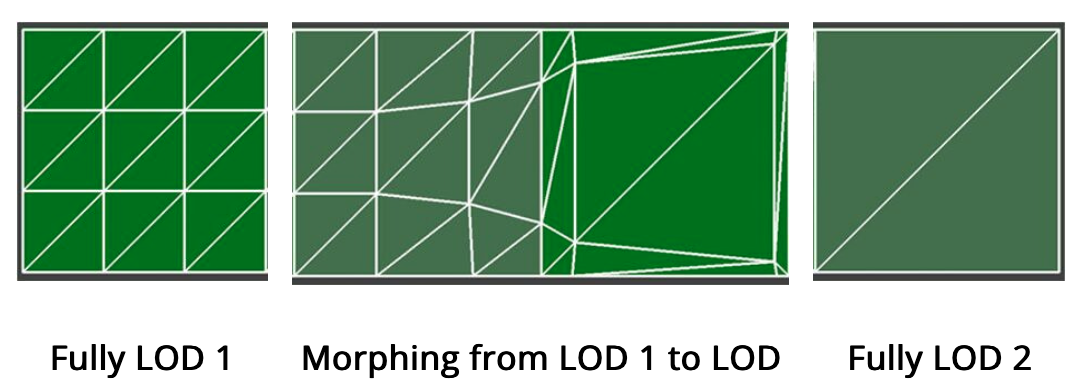
\includegraphics[width=0.8\textwidth]{unreal-morph}
  \caption{Unreal Engine's landscape system LOD morphing (taken from \cite{unrealengine5doc}).}\label{fig:unreal-morph}
\end{figure}

Distant areas get streamed from and to the disk as the camera approaches 
or leaves them, respectively. 

\subsubsection{Frostbite}
Frostbite is a closed-source game engine developed by DICE and is known for the \textit{Battlefield} series.
DICE has held numerous talks in the last few years describing iterations of their
terrain system.

In 2007, Andersson at DICE published a paper describing the terrain rendering 
of the Frostbite game engine. Their approach stores a flat mesh of size $33 \times 33$
in a single vertex buffer, which gets and translated to its actual position at runtime.
The heightmap is stored in a texture image and sampled in the vertex shader, similarly to 
\cite{gpugeomclipmaps}. The view-frustum culling is performed with a quadtree 
and cracks in the terrain get avoided in a similar way to \cite{geomipmapping},
except that crack-causing vertices get removed in the higher resolution mesh,
rather than in the lower resolution mesh. This means that only
9 permutations of the mesh need to be stored, rather than 16.

During the Game Developers Conference 2012, Widmark DICE presented the terrain system of \textit{Battlefield 3}, which was developed with their Frostbite 2 engine \cite{bf3}.
The system is a quadtree-based terrain LOD system and improves on their previous work with a greater focus on paging and streaming of terrain data.
